%!TEX root = pcp.tex

\section{Branch and Cut}
\label{sec:bnc}

In this section we will present the implemented branch-and-cut algorithm, including all the components that compose the branch and cut structure, such as initial heuristic, branching strategies, separation algorithms and primal heuristics.

\subsection{Algorithm structure}

The structure of a branch and cut algorithm can be considered a combination of cutting planes and branch and bound schemes, which we describe below.

\subsubsection*{Cutting planes}

Cutting planes algorithms rely solely on valid inequalities for solving the problem. Given a solution of the model's linear relaxation \footnote{The linear relaxation of an integer linear programming consists in removing all integrality constraints on the variables.}, cutting planes are added to the formulation in order to remove the fractional solution obtained. 

Recall that valid inequalities have the property of being satisfied by all integral solutions of the model, but not necessarily by all fractional solutions in the relaxation; therefore, given a fractional solution $x^*$, there is a cutting plane generated by a linear inequality that holds for all integral solution but is not satisfied by $x^*$. 

The algorithm consists in repeating this process, re-solving the relaxation with all added cuts in each iteration, until an integer-feasible solution is obtained.

\begin{algorithm}
\caption{General scheme for a cutting planes algorithm}
\label{alg:cuttingplanes}

\begin{algorithmic}

\LOOP
	\STATE calculate solution of the linear relaxation
	\IF{solution is integral}
		\RETURN obtained solution
	\ENDIF
	\STATE generate a set of cutting planes to cut off the fractional solution
	\STATE add the cutting planes to the model
\ENDLOOP

\end{algorithmic}
\end{algorithm}

The algorithm depends on having an adequate set of cutting planes families, along with good separation heuristics, in order to find valid inequalities that cut off the relaxation's fractional solution on every iteration. Excessive generation of cutting planes may have the drawback that the relaxation becomes larger and larger on every iteration, requiring a greater computational effort to solve.

Note that, besides the valid inequalities specific to each problem, such as the ones we have presented for \PCP{} in section \ref{sec:ineqs}, there are generic families of cutting planes that can be applied to any problem. However, problem-specific cuts usually have better performance than generic ones.

\subsubsection*{Branch and bound}

The branch and bound scheme explores different solutions by setting bounds on fractional variables on every partial solution. The algorithm starts by solving the relaxation, like cutting planes, but instead of removing the fractional solution by adding a valid inequality, it creates two subproblems, usually by fixing a particular variable with a fractional value to either zero or one. 

Each subproblem is then solved using the same strategy until the relaxation's solution is integer feasible, in which case that branch is closed; note that eventually all variables are fixed to an integer value, so an integer solution is always found. The algorithm runs until all nodes are explored.

Besides the \textit{branching} behaviour of the algorithm, both upper and lower \textit{bounds} for each node are considered. A global upper bound (in case of a minimization problem) is updated whenever a new integer feasible solution is found, keeping the one with the lowest objective value. This upper bound is compared with each node's lower bound provided by the relaxation's solution. Since the integer solution will always be greater than the relaxation's, when the lower bound of the node is larger than the global upper bound, the branch can be pruned.

\begin{algorithm}
\caption{General scheme for a branch and bound algorithm}
\label{alg:branchnbound}

\begin{algorithmic}

\STATE initialize \textit{tree} with the problem's formulation
\STATE 
\WHILE{there are open nodes in the \textit{tree}}
	\STATE pick an open \textit{node} from the tree
	\STATE calculate solution $x^*$ of the linear relaxation of the \textit{node}
	\IF{the linear relaxation is infeasible}
		\STATE close the node as the branch is infeasible
	\ELSIF{solution $x^*$ is integer feasible}
		\STATE update best integer solution $x_M$ with $x^*$ if $f(x^*) < f(x_M)$
		\STATE close the node as an integer solution was found
	\ELSIF{$f(x^*) > f(x_M)$} 
		\STATE close the node as best solution cannot be improved
	\ELSE
		\STATE generate new subproblem nodes by \textit{branching}
	\ENDIF
\ENDWHILE

\RETURN best integer solution $x_M$

\end{algorithmic}
\end{algorithm}

The branch and bound scheme does not specify which node to select on each iteration, or how to generate the subproblems on each node. The selection strategy and the branching strategy are chosen depending on the problem to solve.

\subsubsection*{Cut and branch}

The cut and branch scheme is simply an execution of the cutting planes algorithm until a certain threshold is reached (expressed in running time, number of cuts iterations or mip gap). Then the generation of cutting planes is stopped and a branch and bound algorithm is executed, using the initial formulation augmented with all the generated cutting planes.

This algorithm usually yields better results than the previous ones, as cutting planes may have difficulties finding inequalities that remove fractional solutions very close to the convex hull, and a pure branch and bound scheme usually takes too long to solve as the enumeration may be too large. However, since the cutting planes may cause that the relaxations in the branch and bound become tougher to solve, a good balance between the two phases is extremely important for a good overall performance.

\subsubsection*{Branch and cut}

While the cut and branch algorithm applies cutting planes only at the root of the branch and bound tree, the branch and cut version uses cutting planes throughout the whole tree. Although cuts are applied more aggressively at the root, on certain internal nodes more iterations of cuts are executed. 

Note that these generated cuts can use local information, exploiting the variables fixed in the node due to the branching process. In this case, cuts generated on the node are only valid on the node and its subtree; otherwise, cuts generated on an internal node may be reused globally.

An improvement to this scheme consists in deriving integral solutions from node relaxations, obtaining global upper bounds earlier during the traversal, which allow to prune branches earlier. The generation of these solutions is done via \textit{primal heuristics}.

As with all previously mentioned algorithms, branch and cut schemes have a number of parameters and strategies to determine. To begin with, all the separation heuristics for cutting planes iterations must be chosen adequately to quickly find a reasonable number of cuts; on the branch and bound side, node selection and branching strategies must also be determined. Also, the number of cut iterations to perform on the root and on internal nodes must be set, as well as choosing on which nodes cutting planes and primal heuristics should be executed.

Throughout this section we will go over all these missing pieces in the branch and cut structure, and point out how we filled them in the context of the partitioned coloring problem.

\subsection{Preprocessing}

The first step in solving a \PCP{} instance consists in preprocessing the graph, applying all the following rules until no more modifications are made to the graph:

\begin{enumerate}
	\item{As an initial step, every edge with both ends within the same partition is removed. Since only one node is colored per partition, there can be no color conflicts between nodes of the same partition, and all edges connecting them can be removed, in order to greatly reduce the size of the graph and the number of adjacency restrictions generated.}
	\item{Partitions containing isolated nodes can be completely removed from the graph, as any isolated node can be trivially colored using the lowest possible label, and coloring a single node within a partition marks the whole partition as colored, therefore allowing us to completely remove it.}
	\item{Neighbourhood inclusion criteria is applied within a single partition in order to remove higher-order nodes. Let $u,v$ be two different nodes in a partition $P_k$, if $N(u) \subseteq N(v)$, then we can remove node $v$ from the graph. Since only one node per partition needs to be colored, any valid coloring that assigns color $j_0$ to node $v$ can be modified to assign color $j_0$ to node $u$ instead, still satisfying all color constraints. Intuitively, we are removing \textit{difficult} nodes from a partition when we find an easier one to substitute it. See figure \ref{fig:neighbourinclusion} for an example.}
	
\begin{figure}
	\centering
	\begin{tikzpicture} 
		[includer/.style= {minimum size=3mm,thick,circle,draw=red!75,fill=red!20}, 
		included/.style= {minimum size=3mm,thick,circle,draw=green!75,fill=green!20}, 
		other/.style= {minimum size=3mm,thick,circle,draw=black,fill=black}, 
		transition/.style={thick,draw=black,fill=black!20}] 
		
		\node[other] (n3) at ( -1,3) {}; 
		\node[other] (n4) at ( 0,3) {}; 
		\node[other] (n5) at ( 1,3) {}; 
		\node[other] (n6) at ( 2,3) {}; 
		
		\node[includer] (n1) at ( 0,0) {$v_1$}
			edge [-]	(n3)
			edge [-]	(n4)
			edge [-]	(n5)
			edge [-]	(n6)
		;
		
		\node[included] (n2) at ( 1,0) {$v_2$}
			edge [-]	(n4)
			edge [-]	(n5)
			edge [-]	(n6)
		;
		
	
		\begin{pgfonlayer}{background} 
			\node [fill=black!10,circle,fit=(n1) (n2),label=350:$P_1$] {}; 
		\end{pgfonlayer} 
		
	\end{tikzpicture} 
\caption{Neighbourhood inclusion example: node $v_1$ will be removed from the graph as its neighbourhood completely contains $N(v_2)$.}
	\label{fig:neighbourinclusion}
\end{figure}
	
	\item{A lower bound for the chromatic number of the graph is obtained by finding a maximal clique in the partitions graph $G'$. Finding a clique of size $\omega$ in $G'$ implies that at least $\omega$ different colors are needed for coloring the partitions graph, and the same lower bound clearly holds for $G$. All partitions in the clique will have their colors fixed to $1,\ldots,\omega$ in order to reduce the number of possible colorings, since each of them must be painted using a different color.}
	\item{As in step 2, partitions that contain at least one node with degree less than the lower bound found in the previous step are removed. A node with strictly less than $\omega$ neighbours can be assigned a color among $1,\ldots,\omega$, knowing that no color conflicts will occur; and since there are already $\omega$ colors required, the chromatic number is not increased by that assignment, and therefore the node can be discarded.}
\end{enumerate}

Last 3 steps are performed until no more changes are made to the graph. The resulting largest clique found is used to fix the colors of the partitions included in it. 

Every step is processed by brute force, since their running time is polynomial in the size of the graph, except for step 4 for which we use the algorithm presented below.

\subsubsection*{Partitions graph clique detection}

To find the maximum clique in the partitions graph we use a simple backtracking algorithm. Since the running time of this algorithm can be excessive for a preprocessing step, we bound the running time of this algorithm to five seconds; however, the algorithm usually ends much sooner, as the partitions graph is not only smaller but also much less dense than the original graph. 

In case the time bound is reached, the best solution found so far is returned. As the backtracking uses DFS to explore all possible solutions, a reasonably good solution is generated early in the algorithm, therefore a valid result is obtained regardless its interruption.

Starting with an initial node, the algorithm keeps a list of valid candidates for the clique, which is updated on each iteration by removing all nodes that are not adjacent to the clique. Keeping both the candidates list and all adjacency lists sorted by degree makes computing the intersection between these lists faster, and produces better initial solutions that can be used to prune other solutions later.

\begin{algorithm}
\caption{Finding a maximum clique in a simple graph $G=<V,E>$}
\label{alg:gpclique}

\begin{algorithmic}

\STATE sort all nodes and adjacency lists descendingly by degree

\FORALL{initial node $v$ in $V$}
	\STATE initialize \textit{clique} with node $v$
	\STATE initialize \textit{candidates} with $N(v)$
	\CALL clique 
\ENDFOR

\PROC{clique}
	\IF{\textit{candidates} is empty}
		\STATE update \textit{best} solution if current \textit{clique} is better
	\ELSIF{\textit{clique}.size + \textit{candidates}.size $\leq$ \textit{best}.size}
		\STATE prune current tree
	\ELSE
		\STATE pop node $u$ from \textit{candidates} and add it to \textit{clique}
		\STATE intersect \textit{candidates} with $N(u)$ and store \textit{removed} nodes
		\CALL clique
		\STATE remove node $u$ from \textit{clique}
		\STATE add \textit{removed} nodes back to \textit{candidates} 
		\CALL clique
	\ENDIF
\ENDPROC

\end{algorithmic}
\end{algorithm} 

\subsection{Initial heuristic}

A good initial heuristic solution gives an upper bound on the solution, eliminates a large number of variables and restrictions in the model, and can be used as an initial incumbent solution for the branch and cut algorithm. 

In order to generate this solution, we use the modification of the \textsc{dsatur} algorithm for partitioned graphs presented in \ref{sec:heur}. Since the algorithm generates an implicit enumeration of all possible colorings, which might take too long to compute, its running time is bounded to five seconds. The coloring of the partitions in the clique $K$ is fixed to labels $1, \ldots, \omega$ in order to reduce the solutions set.

\subsection{Initialization}

Using the initial solution as an upper bound $\hat{\chi}$ for the chromatic number, it is possible to eliminate all $x_{ij}$ and $w_j$ variables with $j > \hat{\chi}$, thus greatly reducing the number of involved variables and restrictions in the model.

Another optimization is to fix the colors for all partitions involved in the clique $K$ found during the preprocessing stage. Since it is not possible to determine which node within the partition is to be colored, we simply set to zero all $x_{ij}$ variables for nodes within the partitions that use a different color than the one assigned. Formally, let $K = \{ P_{K_1}, \ldots, P_{K_\omega} \}$ be the initial clique, then:
\begin{align*}
x_{ij} = 0 \quad &\forall i \in K[l],\ \forall 1 \leq l \leq \omega,\ \forall j \neq l \\
w_j = 1 \quad &\forall 1 \leq j \leq \omega
\end{align*}

Also, in case the partition being fixed to a color $j_k$ has a single node in it, then variable $x_{ij_0}$, where $i$ is the single node in the partition, is fixed to $1$.

Another bound based on nodes degree is imposed. A node $v$ of partition degree $\delta_P(v)$ can always be colored with a label $j_k$ such that $1 \leq j_k \leq \delta_P(v) + 1$, since it will be neighbour to at most $\delta_P(v)$ different colors, therefore any set of $\delta_P(v) + 1$ colors contains at least one valid label that does not generate color conflicts.  
\begin{equation*}
x_{ij} = 0 \quad \forall i \in V,\ \forall 1 \leq j \leq \delta_P(v) + 1 \\
\end{equation*}

Finally, in case minimum partition index breaking symmetry restrictions (\ref{eqn:minlabel}) are being used, this is, the color with the lowest label is assigned to the color class containing the partition with the lowest index, another bound can be imposed on $x_ij$ variables. Since in the worst case all partitions will have a different color, then a partition with index $k$ will never be colored with label greater than $k$. Therefore, the following bound is imposed:
\begin{equation*}
x_{ij} = 0 \quad \forall P_k \in P,\ \forall i \in P_k,\ \forall j > k \\
\end{equation*}

\subsection{Cuts separation}

For each family of valid inequalities listed in \ref{sec:ineqs}, an heuristic is implemented to find a set of valid inequalities being violated in a given linear relaxation of the model. Note that in most cases, finding all violated inequalities in a solution is NP, so heuristic procedures must be applied. 

Since these algorithms are applied frequently during the branch and cut tree, it is imperative that their running time is as fast as possible, in order to minimize the added overhead to the whole algorithm.

\subsubsection*{Extended clique cuts}

Separation of extended clique cuts (\ref{ineq:extendedclique}) is done using a very similar algorithm to \ref{alg:gpclique}, adapted to partitioned graphs and without backtracking, so running time is acceptable for a separation algorithm. This algorithm is executed once for each color, and nodes are sorted based not on their degree but on their $x_{ij}$ value in the current solution.

For each initial node, a clique is constructed until the corresponding inequality is broken, and extended to up to $\kappa$ maximal cliques using backtracking, making use of the \textit{candidates} collection (note that in this case, \textit{candidates} is initialized with not only the initial node's neighbours, but also with all the nodes in its partition). In case no clique breaking the inequality is found, the next initial node is picked.

In order to avoid exploring the same solution space multiple times for different initial nodes, restrictions on how many times a node or an edge can be visited are applied. The resulting algorithm is presented in \ref{alg:sep:extclique}.

\begin{algorithm}
\label{alg:sep:extclique}

\begin{algorithmic}

\FORALL{color $j$ such that $w_j \geq \mu$}
\STATE sort all nodes and adjacency lists descendingly by $x_{ij}$ value
 
\FORALL{initial node $v$ in $V$}
	\STATE initialize \textit{clique} with node $v$
	\STATE initialize \textit{candidates} with $N(v) \cup P(v)$

	\WHILE{\textit{candidates} is not empty}
		\IF{current clique breaks inequality}
			\FORALL{maximal cliques $K$ containing \textit{clique} up to $\kappa$}
				\STATE add extended clique cut using $K$ and color $j$ 
			\ENDFOR
			\CONTINUE with next initial node
		\ELSIF{next candidate $u$ can be used}
			\STATE add $u$ to \textit{clique} and remove it from \textit{candidates} 
			\STATE remove nodes not adjacent to $u$ from \textit{candidates} 
		\ELSE
			\STATE remove $u$ from \textit{candidates}
		\ENDIF
	\ENDWHILE
		
\ENDFOR
\ENDFOR

\caption{Separation algorithm for extended clique cuts}

\end{algorithmic}
\end{algorithm} 

\subsubsection*{Component independent set inequalities}

Component hole \ref{ineq:chole} and component path \ref{ineq:cpath} inequalities are separated within the same procedure using a greedy heuristic. In a similar fashion to algorithm \ref{alg:sep:extclique}, for every color the graph is sorted according to $x_{ij}$ values, and for each initial node a component path or hole is greedily constructed. Once again, bounds for a maximum number of visits on each node are imposed, thus rejecting nodes with a certain number of visits or belonging to a partition already in the path, since this would violate the \textit{component} property.

On every iteration the most promising node is added to the path being built. In case this node is adjacent to a node already in the path (thus generating a hole), it is added only if it violates the corresponding inequality, otherwise, the next candidate is picked, and so forth. Algorithm \ref{alg:sep:ciset} resumes this process.

\begin{algorithm}
\label{alg:sep:ciset}

\begin{algorithmic}

\FORALL{color $j$ such that $w_j \geq \mu$}
\STATE sort all nodes and adjacency lists descendingly by $x_{ij}$ value
 
\FORALL{initial node $v$ in $V$}
	\STATE initialize \textit{path} with node $v$

	\LOOP
		\FORALL{valid node $u$ adjacent to last node in the path}
			\IF{$u$ is adjacent to a previous node $w$ in the path}
				\IF{hole $H=[u,\ldots,w]$ violates inequality \ref{ineq:chole}}
					\STATE add component hole inequality with hole $H$ and color $j$
					\CONTINUE with next initial node
				\ENDIF
			\ELSE
				\STATE add node $u$ to \textit{path}	
				\IF{current \textit{path} breaks inequality \ref{ineq:cpath}}
					\STATE add component path inequality with \textit{path} and color $j$
					\CONTINUE with next initial node
				\ENDIF
			\ENDIF
		\ENDFOR
	\ENDLOOP
\ENDFOR

\ENDFOR

\caption{Separation algorithm for component independent set cuts}

\end{algorithmic}
\end{algorithm}

As an alternative to the previous algorithm, we also implemented the hole detection algorithm presented in \cite{nikolopoulos2004hole}. We adapted the algorithm presented in the paper to reject a node if it belongs to a partition already in the path, therefore exploring only component holes; and tested this implementation against the previous one in section \ref{sec:results}.

\subsubsection*{Partitions graph independent set inequalities}

For both path and hole inequalities (\ref{ineq:gpiset}) over the partitions graph $G'$, algorithms equivalent to the ones used for component independent sets are applied as separation heuristics.

Graph $G'$ is constructed once at the beginning of the branch and cut and is then used as input for these heuristics. Since there are no $x_{ij}$ variables to use for sorting the nodes of the graph, the value $\sum_{i \in P_k} x_{ij}$ is used for each partition $P_k$, this is, the sum of the values of the partition's nodes.

\subsubsection*{Block color inequalities}

Block color inequalities (\ref{ineq:blockcp}) are explored using brute force, since there are no more than $c \times q$ of them, and checking whether they are violated or not can be performed fast enough.

Alternatively, they can be added initially to the cut pool provided by the branch and cut framework, instead of manually checking them at each cuts iteration.

\subsection{Node selection strategies}

On each iteration of the branch and cut algorithm, an unprocessed node must be chosen to be solved. Determining which node will be handled next is known as the \textit{node selection} strategy.

There are different standard node selection strategies, all of them implemented by the branch-and-cut framework we used. In section \ref{sec:results} we experiment with the behaviour of the algorithm under different strategies:
\begin{itemize}
	\defitem{DFS}{Depth-first search, picks the last node opened, attempting to generate an integral solution by diving to the bottom of the tree as fast as possible. This strategy has low memory consumption as relatively few nodes are left unprocessed on every iteration.}
	\defitem{BFS}{Breadth-first search, picks the first node opened; this strategy solves every open node with at the same depth before proceeding to the following depth level. It usually has memory issues, as a large number of nodes tend to be left open, thus making this a poor choice in most cases.}
	\defitem{BestBound}{Best-bound, picks the open node with best objective function available, thus closer to an integer feasible solution. This strategy usually reports the best results.}
	\defitem{BestEstimate}{Best-estimate uses \textit{an estimate of a given node's progress toward integer feasibility relative to its degradation of the objective function}\cite{cplex121}; it improves the chance of finding feasible solutions when they are difficult to generate, which is not the case in \PCP{}.}
\end{itemize}


\subsection{Branching strategies}
\label{subsec:alg:branching}

After each node in the branch and cut tree is processed, new child nodes are created by subdividing the problem into two easier subproblems; this is usually done by \textit{branching} on a certain variable. Usually, in the case of binary variables, a variable $x$ with a fractional value in the relaxation is chosen, and the two subproblems are created by fixing $x = 0$ and $x = 1$ and re-processing. Alternatively, bounds on expressions, instead of on variables, can be set.

\begin{figure}[h]
	\label{fig:branching}
	\centering
	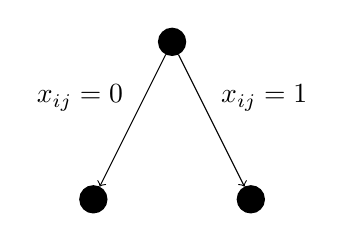
\begin{tikzpicture} 
		[black/.style= {minimum size=3mm,thick,circle,draw=black,fill=black},
		 branch/.style= {->}] 
		
		\node[black] (n1) at ( 0,0) {};
		\node[black] (n2) at ( 2,0) {};
		
		\node[black] (n3) at ( 1,2) {}
			edge[branch] node[swap,auto] {$x_{ij} = 0$} (n1)
			edge[branch] node[auto] {$x_{ij} = 1$} (n2)	
		;
		
	\end{tikzpicture} 
\end{figure}

Whichever method of branching is chosen, it requires that the solutions represented by the union of all subproblems cover all integral solutions represented by the parent node; otherwise, feasible solutions may be left unexplored.

Choosing which variable to branch on, and what bounds are implied within each branch, is part of what is called the branching strategy. 

\subsubsection*{Static priorities}

The simplest way to choose which variable to branch on is to assign a priority to each $x_{ij}$, which will be used to pick the branching variable when necessary: the integer infeasible variable with the highest priority is picked on every branching. 

We experimented in section \ref{subsec:resultsbranching} with combinations of the following criteria for selecting variable $x_{ij}$:

\begin{itemize}
\item{The number of partitions adjacent to node $i$}
\item{The size of the partition containing node $i$}
\item{The label of color $j$}
\end{itemize}

Using this criteria has the huge drawback that no information regarding the actual value of the $x_{ij}$ variable is used, so these priorities work best as a tie-breaker for another strategy.

\subsubsection*{Fractional values}
\label{subsubsec:alg:branch:frac}

A common practice is to pick the most fractional variable to branch on. We determine such variable as:
\[
\min_{x_{ij}} \{ |x_{ij} - 0.5| \}
\]

In case of a tie, we use the static priority set for the variables to determine which one use to branch on. We also experimented in section \ref{subsec:resultsbranching} with the opposite criteria, this is, branching on the less fractional value (excluding those variables with already integral values).

This is a common branching technique, but does not exploit any particular feature of the problem being studied, unlike the one described below.

\subsubsection*{Degree of saturation}
\label{subsubsec:alg:branch:dsatur}

A branching strategy specifically related to the partitioned coloring problem is to branch on a node with the highest degree of saturation. Since these nodes are usually the most difficult ones to handle, it is reasonable to fix their values as early as possible in the branch and cut tree.

This criteria for picking the branching variable requires first to compute an approximate degree of saturation for every node and choosing the one with the largest value, $i^*$, in order to obtain a set of candidate variables $x_{i^*j_0}, x_{i^*j_1}, \ldots, x_{i^*j_c}$ (once again, ties between nodes are broken using the already defined priorities).

Since the only available values are those of the fractional solution, we color one node in each partition using the largest value within the partition and neighbours: this is, for every node $i$ and color $j$ combination, if the value $x_{ij}$ is larger than all of its neighbours and nodes in the same partition, as well as larger than an arbitrary lower bound ($0.7$)\footnote{Note that if the classic constraints are being used, \ref{eqn:partsum} and \ref{eqn:adjscolorp}, by specifying a lower bound higher than $0.5$ it is not necessary to verify that the node has the highest value among its neighbours or within the partition, as it will be assured by the restrictions; the check is required in case alternative restrictions are used, such as allowing more than one node to be colored or grouping multiple color conflicts into single constraints.}, we assign color $j$ to node $i$. Note that some partitions might be left uncolored, in this case they will not contribute to the degree of saturation of their neighbours.

\begin{equation}
\label{eqn:fixcriteria}
v_i \leftarrow j \text{ if } x_{ij} > 0.7 \wedge x_{ij} > x_{kj}\ \forall k \in N(i) \cup P(i)
\end{equation}

\begin{nuevo}
Having chosen a node $v_i$ for branching, we must choose which variable $x_{i^*j^*}$ from the set of candidate $x_{i^*j_0}, x_{i^*j_1}, \ldots, x_{i^*j_c}$ will be branched on. We have implemented two different strategies for this:
\begin{itemize}
	\defitem{\textsc{dsatur-2}}{Choose the variable $x_{i^*j^*}$ with the highest value from the set, and branch on $x_{i^*j^*} = 0$ and $x_{i^*j^*} = 1$; this results in a classic $0-1$ branching on the variable corresponding to the most saturated node with its most \textit{likely} color.}
	\defitem{\textsc{dsatur-(C+1)}}{Create up to $C+1$ subproblems, one for each possible coloring of the node, branching on $x_{i^*j_0} = 1, \ldots, x_{i^*j_c} = 1$, plus another child which sets all $x_{i^*j_0}$ variables to zero, in case the node is not colored within its partition.}
\end{itemize}
\end{nuevo}

\sout{
From the mentioned set of candidates $x_{i^*j_0}, x_{i^*j_1}, \ldots, x_{i^*j_c}$, the variable with the highest value is chosen for branching. Overall, we are branching on the node with the highest degree of saturation, fixing it to the most probable color it was assigned in the relaxation.
}

\subsubsection*{Implied bounds}
\label{subsubsec:alg:branch:bounds}

When manually specifying the branching variable and creating the subproblems, it is also possible to fix more variables that would be affected by the value assigned to the first one.

Regardless of the branching variable, it is possible to fix all color variables $w_j$ to $1$ for $j = 1,\ldots,\ceil{z}$, where $z$ is the value of the objective function of the current node's relaxation. For example, if the sum of all $w_j$ variables is $5.3$, which is a lower bound on the chromatic number, we can be sure that at least $6$ different colors are needed to color the graph, and therefore all $w_1,\ldots,w_6$ can be set to $1$.

When branching down on the selected variable\footnote{Fixing the branch variable's value to 0.}, there are no more logical implications than the previous one that can be used to bound more variables. This is easy to see since setting an $x_{ij}$ variable to zero implies that a certain color will not be used for a certain node, but does not grant any information on which \textit{node} on the partition will be colored and with which \textit{color}.

Branching up, on the other hand, provides much more information. Whenever a variable $x_{i^*j^*}$ is set to $1$, this is, node $i^*$ in partition $P(i^*)$ is assigned color $j^*$, we may specify the following conditions for that branch:

\begin{itemize}
\item Every other color-node combination in partition $P(i^*)$ can be set to zero, as only one node must be assigned a color in the partition.
\[
x_{ij} = 0 \quad \forall i \in P(i^*),\ \forall j \in C,\ i \neq i^* \vee j \neq j^*
\]

\item Every node adjacent to $i^*$ cannot use color $j^*$ in order to avoid color conflicts.
\[
x_{ij^*} = 0 \quad \forall i \in N(i^*)
\]
\end{itemize}

\subsection{Primal heuristic}
\label{subsec:alg:primal}

The algorithm used to create an integer feasible solution from the relaxation's solution is called the \textit{primal heuristic}. A typical primal heuristic consists in rounding the values of every fractional variable to the nearest integer value, as long as this process satisfies all the restrictions imposed by the model.

For \PCP{} we implemented a primal heuristic based on the \textsc{dsatur} algorithm. Given a fractional solution $x^*$, for every variable $x_{ij}$ with a large enough value, we fix that node-color combination. The criteria used for determining when a variable is fixed is the same as the one depicted in \ref{eqn:fixcriteria}.

Also, for every variable $x_{ij}$ with an upper bound set to $0$ as a product of the branching in the branch and cut tree, we forbid that node-color combination.

Having all these values fixed, an extremely short run of \textsc{dsatur} is executed, bounded to 200 milliseconds. The algorithm works reasonably fast as more and more variables are fixed, and bounds for the optimal coloring can be inferred from the branch and cut tree, further shortening the exploration of possible solutions. 
\begin{itemize}
\item{Value $\ceil{\sum_{j \in C} w_j}$ of the node's relaxation is a lower bound to the integer solution, so in case \textsc{dsatur} finds a solution using that number of colors, it can be assured that it is the local optimum.}
\item{The solution of the primal heuristic will be used as the global upper bound, replacing the current incumbent solution, only if it uses less colors. Therefore, \textsc{dsatur} is bounded to exploring solutions that use strictly less colors than the incumbent.}
\end{itemize}

The best coloring obtained by the algorithm is then used as an incumbent solution for the node. In case certain symmetry breaking restrictions are in place, a reordering of the labels assigned to each color class might have to be performed.

\subsection{Implicit enumeration}
\label{subsec:alg:implicit}

Early experimentation with the branch and cut algorithm and with the \textsc{dsatur} algorithm has shown that, for relatively small instances, the latter explores all possible solutions much faster than the former, since it does not have all the overhead imposed by the different artifacts present in a full branch and cut.

Therefore, when we have reduced the problem size to a relatively small one by fixing node-color assignments during the branching process, instead of proceeding with the traditional branch and cut algorithm, we execute a full run of \textsc{dsatur}. Since most partitions are already colored, the number of possible solutions is reasonably small to be fully explored.

In section \ref{sec:results} we experiment with different values for the number of uncolored partitions in the branch and cut tree to be used as the threshold for stopping the branch and cut and starting an unbounded execution of \textsc{dsatur}.

\subsection{Implementation details}

The branch and cut algorithm was implemented in Java 1.6 using CPLEX version 12.1 both as a branch-and-cut framework and a linear programming solver for relaxations. 

We made use of branch, heuristic and cut callbacks provided by the CPLEX API to manage the branching strategy, inject primal solutions and apply custom cuts on both the root and internal nodes.
\begin{itemize}
\item{The branch callback is invoked once the processing of a certain node has been completed in order to determine how to create the child subproblems; inside this callback we implement the different dynamic branching strategies described in \ref{subsec:alg:branching}. Static priorities are fixed during the initialization of the problem. This callback is also used to prune the branch and cut tree once a certain number of partitions have been fixed in order to proceed with the implicit enumeration from \ref{subsec:alg:implicit}.}
\item{The heuristic callback is invoked after the linear relaxation of a node has been solved, and provides the fractional values from the relaxation's solution to derive an integral feasible solution, using the color degree strategy explained in \ref{subsec:alg:primal}. We make use of this callback to inject the integral solution derived from implicit enumeration (\ref{subsec:alg:implicit}).}
\item{The cut callback is invoked after the linear relaxation is solved; every certain number of nodes the separation heuristics are invoked in an attempt to add planes to cut off the current linear solution. After the cuts are added, the relaxation is solved again, and more iterations of cutting planes may be optionally executed; while few iterations are performed in the internal nodes, a larger number is executed in the root.}
\end{itemize} 

The framework was configured to use standard branch and cut search, instead of dynamic search, to correctly determine the performance of the developed strategies. Multi-core processing was also disabled.